\documentclass{article}
\usepackage[utf8x]{inputenc}
\usepackage{ucs}
\usepackage{amsmath} 
\usepackage{amsfonts}
\usepackage{upgreek}
\usepackage[english,russian]{babel}
\usepackage{graphicx}
\usepackage{float}
\usepackage{textcomp}
\usepackage{hyperref}
\usepackage{geometry}
  \geometry{left=2cm}
  \geometry{right=1.5cm}
  \geometry{top=1cm}
  \geometry{bottom=2cm}
\usepackage{tikz}
\usepackage{ccaption}
\usepackage{multicol}

\usepackage{listings}
%\setlength{\columnsep}{1.5cm}
%\setlength{\columnseprule}{0.2pt}


\begin{document}
\pagenumbering{gobble}

\lstset{
  language=C++,                % choose the language of the code
  basicstyle=\linespread{1.1}\ttfamily,
  columns=fixed,
  fontadjust=true,
  basewidth=0.5em,
  keywordstyle=\color{blue}\bfseries,
  commentstyle=\color{gray},
  stringstyle=\ttfamily\color{orange!50!black},
  showstringspaces=false,
  %numbers=false,                   % where to put the line-numbers
  numbersep=5pt,
  numberstyle=\tiny\color{black},
  numberfirstline=true,
  stepnumber=1,                   % the step between two line-numbers.        
  numbersep=10pt,                  % how far the line-numbers are from the code
  backgroundcolor=\color{white},  % choose the background color. You must add \usepackage{color}
  showstringspaces=false,         % underline spaces within strings
  captionpos=b,                   % sets the caption-position to bottom
  breaklines=true,                % sets automatic line breaking
  breakatwhitespace=true,         % sets if automatic breaks should only happen at whitespace
  xleftmargin=.2in,
  extendedchars=\true,
  keepspaces = true,
}
\lstset{literate=%
   *{0}{{{\color{red!20!violet}0}}}1
    {1}{{{\color{red!20!violet}1}}}1
    {2}{{{\color{red!20!violet}2}}}1
    {3}{{{\color{red!20!violet}3}}}1
    {4}{{{\color{red!20!violet}4}}}1
    {5}{{{\color{red!20!violet}5}}}1
    {6}{{{\color{red!20!violet}6}}}1
    {7}{{{\color{red!20!violet}7}}}1
    {8}{{{\color{red!20!violet}8}}}1
    {9}{{{\color{red!20!violet}9}}}1
}

\title{Семинар \#5: Итераторы и контейнеры. \vspace{-5ex}}\date{}\maketitle

\section*{Итераторы}
Контейнер в C++ -- это объект, используемый для хранения других объектов и отвечающий за управление памятью, используемой содержащимися в нем объектами. Примерами контейнеров являются \texttt{std::vector<T>} или \texttt{std::array<T, Size>}.

Итератор - это один из часто используемых паттернов проектирования.
Итератор представляет собой объект, используя который, мы можем получить доступ к элементам некоторого другого объекта.

Итераторы в C++ -- это специальные объекты, которые используются для доступа к элементам контейнеров.
Благодаря им мы можем, например, обойти все элементы контейнера или задать в этом контейнере некоторый диапазон. Для каждого контейнера есть свой тип итератора и этот тип определён внутри самого класса контейнера и называется \texttt{iterator}. То есть, если у нас есть контейнер \texttt{std::vector<int>}, то тип итератора для такого контейнера будет \texttt{std::vector<int>::iterator}.
Также, у каждого контейнера есть специальные методы:
\begin{itemize}
\item \texttt{begin} -- возвращает итератор на первый элемент
\item \texttt{end} -- возвращает итератор на фиктивный элемент, следующий за последним
\end{itemize}
Пример создания итератора вектора и работы с ним:
\begin{lstlisting}
#include <iostream>
#include <vector>
using std::cout, std::endl;

int main()
{
    std::vector<int> v {10, 20, 30, 40, 50};
    std::vector<int>::iterator it = v.begin();
    cout << *it << endl; // Напечатает 10
    it++;
    cout << *it << endl; // Напечатает 20
}
\end{lstlisting}

\subsection*{Операции, которые можно проводить с итератором вектора}

\begin{enumerate}
\item Копирование и присваивание:\quad \texttt{Iterator it1 = it2;} \quad \texttt{it1 = it2}\\
\texttt{it1} будет указывать туда же куда указывает \texttt{it2}.
\item Инкремент/декремент итератора: \quad \texttt{++it} \quad \texttt{it++} \quad \texttt{-{}-it} \quad \texttt{it-{}-}\\
В этом случае итератор начинает указывать на предыдущий или следующий элемент.
\item Прибавление/вычитание целого числа: \quad \texttt{it += k} \quad \texttt{it -= k}\\
В этом случае итератор начинает указывать на элемент, смещённый на это число.
\item Сумма/разность итератора и числа: \quad \texttt{it + k} \quad \texttt{it - k}\\
Результат этой операции - это новый итератор, который смещён на данное число.
\item Вычитание итераторов: \quad \texttt{it1 - it2}\\
Возвращает количество элементов между этими объектами
\item Сравнения:  \quad\texttt{it1 == it2} \quad  \texttt{it1 != it2} \quad  \texttt{it1 < it2} \quad  ...
\item Унарная звёздочка: \quad \texttt{*it}\\
Поставив \texttt{*} перед итератором мы получим объект, на который указывает итератор.
\item Оператор индексирования:\quad \texttt{it[k]}\\
Также, как и для указателей, \texttt{it[k]} это то же самое, что и \texttt{*(it + k)}.
\end{enumerate}     
\textbf{!} Набор операций для других итераторов может сильно отличаться.  

\newpage

\subsection*{Пример прохода по вектору с использованием итератора}
Конечно, можно пройтись по вектору и с помощью обычной целочисленной переменной.
Но можно сделать это и используя итераторы как показано в следующем примере.
\begin{lstlisting}
#include <iostream>
#include <vector>
using std::cout, std::endl;

int main()
{
    std::vector<int> v {11, 22, 33, 44, 55};
    
    // Напечатаем все элементы вектора:
    for (std::vector<int>::iterator it = v.begin(); it != v.end(); ++it)
        cout << *it << " ";
    cout << endl;    
   
    // Увеличим все элементы вектора на 1:
    for (std::vector<int>::iterator it = v.begin(); it != v.end(); ++it)
        *it += 1;
        
    // Напечатаем только чётные элементы:
    for (std::vector<int>::iterator it = v.begin(); it != v.end(); ++it)
    {
        if (*it % 2 == 0)
            cout << *it << " ";
    }
    cout << endl;
}
\end{lstlisting}


\subsection*{Передача итераторов в функции}
С итераторами можно работать как с обычными переменными. Их можно хранить отдельно от контейнера, можно передавать в функции, можно ложить в другие контейнеры и т. д.
\begin{lstlisting}
#include <iostream>
#include <vector>
using std::cout, std::endl;

void print(std::vector<int>::iterator first, std::vector<int>::iterator last)
{
    for (std::vector<int>::iterator it = first; it != last; ++it)
        cout << *it << " ";
    cout << endl;   
}

int main()
{
    std::vector<int> v {11, 22, 33, 44, 55};
    print(v.begin(), v.end());        // Напечатает весь вектор 
    print(v.begin(), v.begin() + 3);  // Напечатает первые 3 элемента 
}

\end{lstlisting}

\newpage
\section*{Контейнеры}
Стандартная библиотека включает в себя множество разных шаблонных контейнеров.

\begin{center}
\bgroup
\def\arraystretch{2}%  1 is the default, change whatever you need
\begin{tabular}{ p{3.3cm} | p{14cm} }
контейнер & описание и основные свойства \\ \hline

\texttt{std::vector} & 
Динамический массив, по умолчанию хранит элементы в куче. \newline 
Все элементы лежат вплотную друг к другу. \newline 
Доступ по индексу за $O(1)$. Вставка/удаление в конец за $O(1)$ в среднем. \newline
В остальных случаях вставка/удаление за $O(n)$. Поиск за $O(n)$.  \newline 
\\ \hline

\texttt{std::array} &
Массив фиксированного размера, хранит элементы в самом объекте. \newline 
Все элементы лежат вплотную друг к другу. \newline 
Доступ по индексу за $O(1)$. Поиск за $O(n)$. \newline 
\\ \hline

\texttt{std::list} &
Двусвязный список \newline 
Вставка/удаление элементов за $O(1)$ если есть итератор на элемент. \newline 
Нет доступа по индексу. Поиск за $O(n)$. \newline 
\\ \hline


\texttt{std::forward\_list} &
Односвязный список \newline 
Вставка/удаление элементов за $O(1)$ если есть итератор на предыдущий элемент. \newline 
Нет доступа по индексу. Поиск за $O(n)$. \newline 
\\ \hline


\texttt{std::deque} &
Двухсторонняя очередь \newline 
Доступ по индексу за $O(1)$. Добавление/удаление в начало и конец за $O(1)$. \newline 
Остальные операции за $O(N)$. \newline 
\\ \hline

\texttt{std::set} &
Реализация множества на основе сбалансированного дерева поиска. \newline 
Хранит элементы без дубликатов, в отсортированном виде. \newline 
Тип элементов должен реализовать \texttt{operator<} (или предоставить компаратор). \newline 
Поиск/вставка/удаление элементов за $O(\log(N))$. \newline 
\\ \hline


\texttt{std::map} &
Реализация словаря на основе сбалансированного дерева поиска. \newline 
Хранит пары ключ-значения без дубликатов ключей, в отсортированном виде. \newline 
Тип ключей должен реализовать \texttt{operator<}  (или предоставить компаратор).\newline 
Поиск/вставка/удаление элементов за $O(\log(N))$. \newline 
\\ \hline


\texttt{std::unordered\_set} &
Реализация множества на основе хеш-таблицы. \newline 
Хранит элементы без дубликатов, в произвольном порядке. \newline 
Поиск/вставка/удаление элементов за $O(1)$ в среднем. \newline 
\\ \hline


\texttt{std::unordered\_map} &
Реализация словаря на основе хеш-таблицы. \newline 
Хранит пары ключ-значения без дубликатов ключей,в произвольном порядке. \newline 
Поиск/вставка/удаление элементов за $O(1)$ в среднем. \newline 
\\ \hline

\texttt{std::multiset} \newline \texttt{std::multimap}
& То же самое, что \texttt{std::set}/\texttt{std::map}, но может хранить дублированные значения  \\
\hline
\end{tabular}
\egroup
\end{center}



\newpage
\section*{Контейнер \texttt{std::list}}
Контейнер \texttt{std::list} реализует двусвязный список.
Его строение можно представлять следующим образом: 

\begin{center}
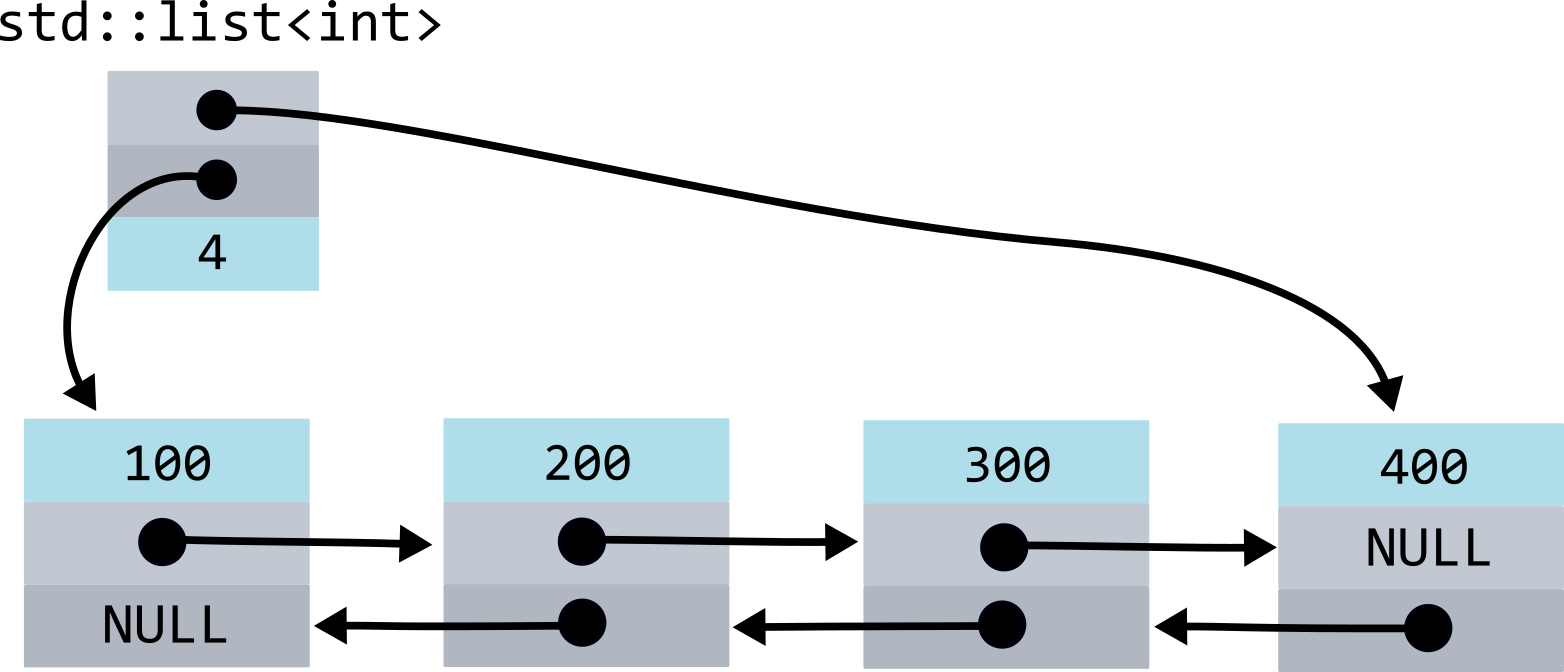
\includegraphics[scale=0.8]{../images/list_internals.png}
\end{center}

 Основные методы для работы со списком. Все перечисленные методы работают за $O(1)$.

\bgroup
\def\arraystretch{2}%
\begin{tabular}{ l | p{8cm} }
метод & описание \\ \hline
\texttt{size\_t size()} & возвращает количество элементов в списке. \newline
                          работает за $O(1)$, так как количество элементов хранится внутри списка.
\\ \hline

\texttt{void push\_back(const T\& el)} & добавляет элемент в конец списка.
\\ \hline
\texttt{void pop\_back()} & удаляет элемент из конца списка.
\\ \hline
\texttt{void push\_front(const T\& el)} & добавляет элемент в начало списка.
\\ \hline
\texttt{void pop\_front()} & удаляет элемент из начала списка.
\\ \hline

\texttt{iterator insert(iterator it, const T\& elem)} & вставляет элемент до элемента на который указывает итератор \texttt{it}. Возвращает итератор на новый элемент.
\\ \hline

\texttt{iterator erase(iterator it)} & удаляет элемент на который указывает \texttt{it}. \newline
                                       возвращает итератор, указывающий на следующий за удалённым. \newline
\\
\end{tabular}
\egroup

Преимущество списка по сравнению с массивом в том, что можно быстро добавлять и удалять элементы в любое место списка (если это положение известно), тогда как в массив можно быстро добавлять/удалять только в конец.

Обратите внимание, что у списка нет оператора индексации \texttt{operator[]},
так как в связном списке нет быстрого способа получить доступ к элементу по его индексу.
Если бы такой метод был бы написан, то он работал бы за $O(n)$, что очень плохо.
Поэтому для обхода связного списка нужно использовать итераторы:

\begin{lstlisting}
#include <iostream>
#include <list>
int main()
{
    std::list<int> a {10, 20, 30, 40};
    a.push_back(50);
    // Напечатаем все элементы списка: 10 20 30 40 50
    for (std::list<int>::iterator it = a.begin(); it != a.end(); ++it)
        std::cout << *it << " ";
    std::cout << std::endl;    
}
\end{lstlisting}



\subsection*{Пример работы со связным списком}
Пример использования методов, описанных выше:
\begin{lstlisting}
#include <iostream>
#include <list>
int main()
{
    std::list<int> a {99, 20, 30, 40, 50};
    
    a.pop_front();
    a.push_front(10);
    
    std::list<int>::iterator it = a.begin();
    it++;
    it++;
    a.insert(it, 99);
    
    // Напечатает 10 20 99 30 40 50
    for (std::list<int>::iterator it = a.begin(); it != a.end(); ++it)
        std::cout << *it << " ";
    std::cout << std::endl;    
}
\end{lstlisting}


\subsection*{Обход связного списка с удалением/добавлением элементов}
Сложность при использовании связного списка и других контейнеров может возникнуть если вы обходите список и при этом его меняете. Например, рассмотрим задачу удаления всех чётных элементов из списка.
\begin{lstlisting}
#include <iostream>
#include <list>
int main()
{
    std::list<int> a {11, 22, 33, 44, 55};
    
    // Неправильный способ. Потому что после удаления элемента итератор на него
    // стал недействительным. Применение ++it к такому итератору приводит к UB.
    for (std::list<int>::iterator it = a.begin(); it != a.end(); ++it)
    {
        if (*it % 2 == 0)
            a.erase(it);
    }
    
    // Правильный способ.
    for (std::list<int>::iterator it = a.begin(); it != a.end();)
    {
        if (*it % 2 == 0)
            it = a.erase(it);
        else
            it++;
    }
    
    for (std::list<int>::iterator it = a.begin(); it != a.end(); ++it)
        std::cout << *it << " ";
    std::cout << std::endl;    
}
\end{lstlisting}


\subsection*{Операции, которые можно проводить с итератором списка}
Набор операций итератора списка значительно меньше, чем у итератора вектора:
\begin{enumerate}
\item Копирование и присваивание:\quad \texttt{Iterator it1 = it2;} \quad \texttt{it1 = it2}\\
\texttt{it1} будет указывать туда же куда указывает \texttt{it2}.
\item Инкремент/декремент итератора: \quad \texttt{++it} \quad \texttt{it++} \quad \texttt{-{}-it} \quad \texttt{it-{}-}\\
В этом случае итератор начинает указывать на предыдущий или следующий элемент.
\item Сравнения на равенство/неравенство:  \quad\texttt{it1 == it2} \quad  \texttt{it1 != it2} \\
Но нельзя сравнивать на больше/меньше.
\item Унарная звёздочка: \quad \texttt{*it}\\
Поставив \texttt{*} перед итератором мы получим объект, на который указывает итератор.
\end{enumerate} 
К итератору списка нельзя прибавлять числа, нельзя вычитать итераторы, сравнивать и применять оператор индексирования. Легко понять почему эти операции для итератора списка не реализованы, если знать внутренее устройство связного списка -- их нельзя реализовать эффективно. Например, операция \texttt{it + n} даже если бы она была реализована, работала бы за $O(n)$, так как, чтобы сместиться вперёд на $n$ элементов в списке, нужно сделать $n$ переходов по указателю.



\section*{Контейнер \texttt{std::forward\_list}}
Контейнер \texttt{std::forward\_list} реализует односвязный список.
Его строение можно представлять следующим образом: 

\begin{center}
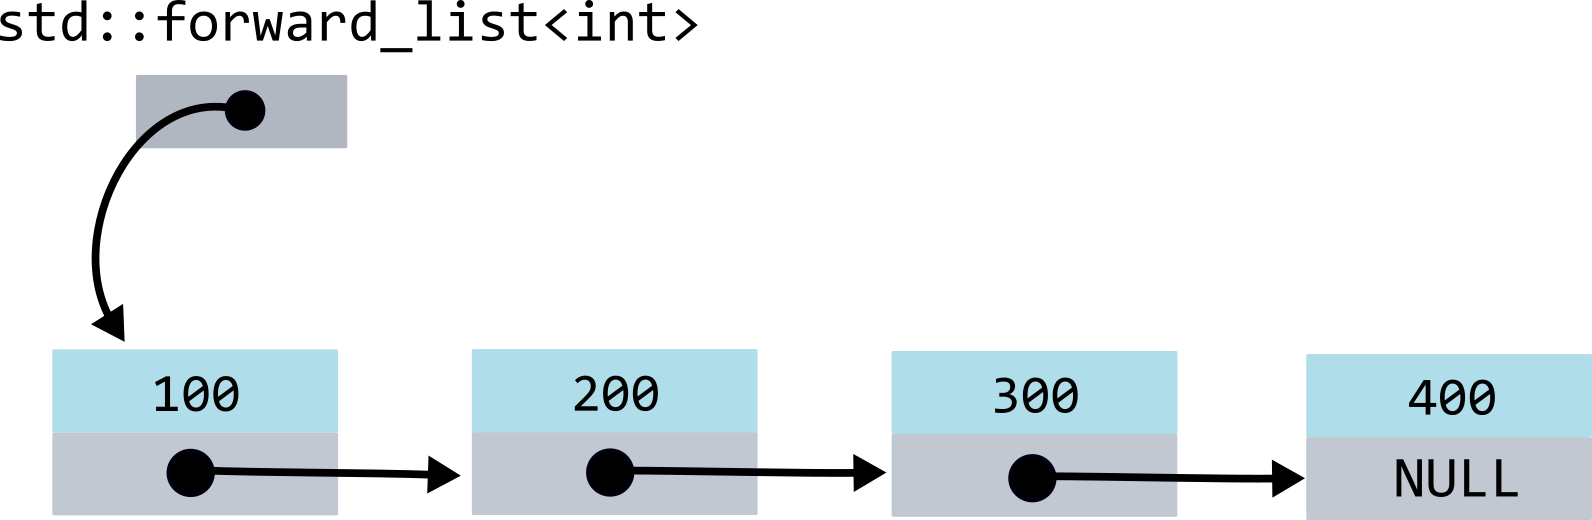
\includegraphics[scale=0.8]{../images/forward_list_internals.png}
\end{center}

Это более легковесный контейнер по сравнению \texttt{std::list}, но менее функциональный.
Например, у него нет методов \texttt{size}, \texttt{push\_back} и \texttt{pop\_back}, а методы \texttt{insert} и \texttt{erase} заменены на \texttt{insert\_after} и \texttt{erase\_after}.


\subsection*{Операции, которые можно проводить с итератором односвязного списка}
Набор операций, которые можно проводить с итератором односвязного списка ещё меньше чем у двусвязного:
\begin{enumerate}
\item Копирование и присваивание:\quad \texttt{Iterator it1 = it2;} \quad \texttt{it1 = it2}
\item Инкремент итератора: \quad \texttt{++it} \quad \texttt{it++}
\item Сравнения на равенство/неравенство:  \quad\texttt{it1 == it2} \quad  \texttt{it1 != it2}\\
Но нельзя сравнивать на больше/меньше.
\item Унарная звёздочка: \quad \texttt{*it}
\end{enumerate} 
В отличии от итератора двусвязного списка к итератору односвязного списка нельзя применять декремент (\texttt{-{}-}).
\begin{lstlisting}
#include <iostream>
#include <forward_list>
int main()
{
    std::forward_list<int> a {10, 20, 30, 40, 50};
    std::forward_list<int>::iterator it = a.begin();
    it++;
    it--; // Ошибка компиляции
}
\end{lstlisting}

\newpage
\section*{Контейнер \texttt{std::set}}
\texttt{std::set} -- это реализация множества с помощью бинарного дерева поиска. Не хранит дупликатов. При попытке добавить в множество тот элемент, который в нём уже есть, ничего не произойдёт. Также все элементы в множестве всегда хранятся в отсортированном виде (так как это бинарное дерево поиска). Для типа элементов множество должен быть реализован \texttt{operator<}. В \texttt{std::set} нельзя менять элементы, так как это бинарное дерево поиска, но можно удалить элемент, а потом вставить новый.\\

\begin{center}
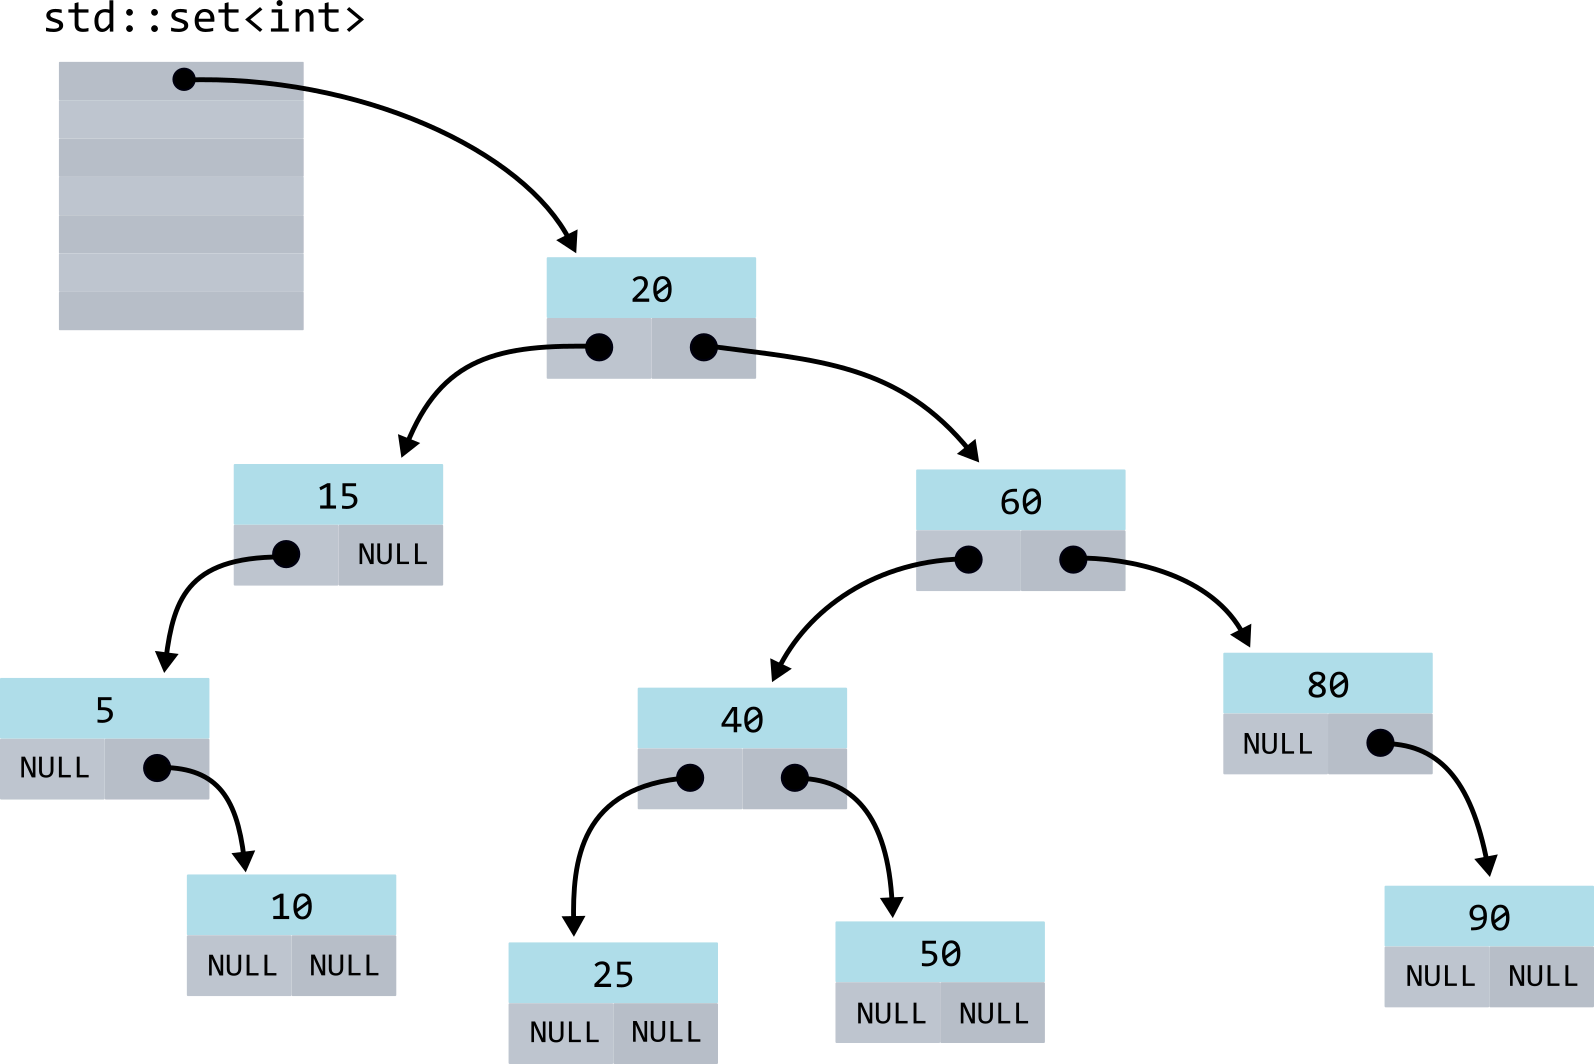
\includegraphics[scale=1]{../images/set_internals.png}
\end{center}

Основные методы для работы с множеством. Все следующие операции работают за $O(log(n))$.

\bgroup
\def\arraystretch{2}%
\begin{tabular}{ p{5cm} | p{12cm} }
метод & описание 
\\ \hline

\texttt{std::pair<iterator, bool> \newline insert(const T\& el)}
& Вставляет элемент в множество \newline
Возвращает пару (итератор, булевое значение). Итератор будет указывать на соответствующий элемент.
Булевое значение будет равно \texttt{true} если вставка была произведена и \texttt{false} если
элемент уже существовал.
\\ \hline

\texttt{iterator erase(iterator it)}  \newline 
\texttt{iterator erase(T\& el)}
& Удаляет элемент. Можно удалять по итератору или по значению элемента.
\\ \hline

\texttt{iterator find(const T\& el)} & Ищет элемент в множестве.\newline
Возвращает итератор на этот элемент или итератор \texttt{end()}, если такого элемента нет.
\\ \hline

\texttt{bool contains(const T\& el)}  & Возращает \texttt{true}, если элемент содержтся в множестве.
\\ \hline

\texttt{iterator lower\_bound(x)}  & Возвращает итератор на первый элемент, который больше или равен \texttt{x}
\\ \hline
\texttt{iterator upper\_bound(x)}  & Возвращает итератор на первый элемент, который больше \texttt{x} \newline
\\
\end{tabular}
\egroup


Преемущество множества над вектором заключается в том, что операции вставки/удаления/поиска работают за $O(log(n))$, что намного быстрее чем у вектора (за исключения вставки/удаления в конец вектора).

Недостатком множества является то, что в нём нельзя быстро найти элемент по индексу.




\newpage
\subsection*{Пример работы с множеством}

\begin{lstlisting}
#include <iostream>
#include <set>

void print_set(std::set<int>::iterator start, std::set<int>::iterator finish)
{
    for (std::set<int>::iterator it = start; it != finish; ++it)
        std::cout << *it << " ";
    std::cout << std::endl;
}

int main()
{
    std::set<int> a {40, 20, 10, 10, 50, 30, 30}; 
    print_set(a.begin(), a.end()); // Напечатает 10 20 30 40 50
    
    a.insert(20);
    a.insert(60);
    a.erase(10);
    print_set(a.begin(), a.end()); // Напечатает 20 30 40 50 60
    
    std::set<int>::iterator it = a.find(50);
    if (it == a.end())
    {
        std::cout << "Element not found" << std::endl;
    }
    else
    {
        std::cout << "Element found. Printing elements starting with this one:" << std::endl;
        print_set(it, a.end());
    }
}
\end{lstlisting}


\begin{itemize}
\item На вход подаётся $n$ чисел. Напечатайте эти числа удалив все дупликаты.
\begin{center}
\begin{tabular}{ l | l }
 вход & выход \\ \hline
 \texttt{10} & \texttt{1 2 7 8}  \\ 
 \texttt{8 2 1 2 2 1 8 7 1 2} &  \\
\end{tabular}
\end{center}



\end{itemize}


\section*{Контейнер \texttt{std::multiset}}
То же самое, что и \texttt{std::set}, но может хранить дупликаты. Одна из неочевидных особенностей \texttt{multiset} это то, что при удалении элемента по значению \texttt{erase(x)}, удалятся все элементы, равные \texttt{x}. Для удаления одного элемента нужно передать в \texttt{erase} итератор на элемент.
\begin{itemize}
\item Считайте $n$ чисел и отсортируйте их с помощью вставки в \texttt{multiset}. Распечатайте отсортированные числа.
\item На прямой лежит верёвка длиной $n$ метров. Затем её начинают последовательно разрезать. Все места разрезов -- целые числа. Найти длину самого длинного куска после каждого разреза.
\begin{center}
\begin{tabular}{ l | l }
 вход & выход \\ \hline
 \texttt{20 8} & \texttt{12 10 8 7 6 5 5 4}  \\ 
 \texttt{8 10 15 1 7 4 11 18} &  \\
\end{tabular}
\end{center}
\end{itemize}

\newpage
\section*{Контейнер \texttt{std::map}}
\texttt{std::map} -- это реализация словаря с помощью бинарного дерева поиска. Не хранит ключей - дупликатов. При попытке добавить в этот словарь элемента с ключом, который в нём уже есть, ничего не произойдёт. Также все элементы в этом словаре всегда хранятся в отсортированном по ключам виде (так как это бинарное дерево поиска). Для типа ключей должен быть реализован \texttt{operator<}. В \texttt{std::map} можно менять значения, но нельзя менять ключи, так как это бинарное дерево поиска. Но можно удалить элемент каким-то ключом, а потом вставить новый с другим ключом.\\

Основные методы для работы с множеством:
\begin{center}
\begin{tabular}{ l | l }
 метод & описание \\ \hline
 \texttt{insert(k, v)}  & Вставляет элемент с ключом \texttt{k} и значением \texttt{v}\\
                        & Если такой элемент уже есть, то ничего не делает \\ \\\hline
 \texttt{operator[]}    &  Вставляет элемент с ключом \texttt{k} и значением \texttt{v}\\
 \texttt{m[k] = v}      & Если такой элемент уже есть, то меняет его значение \\ \\\hline
 \texttt{erase(k)}      & Удаляет элемент. Можно удалять по значению элемента или по итератору.  \\ 
                        & Также можно сразу удалить диапазон значений, если передать 2 указателя \\\\ \hline
 \texttt{find(x)}       & Принимает на вход значение \texttt{x} и ищет элемент с таким ключом. Возвращает итератор на \\
                        &  этот элемент или итератор \texttt{end()}, если такого ключа нет\\ \\ \hline
 \texttt{count(x)}      & Принимает значение и находит, сколько ключей равны этому значению (т.е. 0 или 1) \\ \\\hline
 \texttt{lower\_bound(x)}  & Возвращает итератор на первый элемент, который больше или равен \texttt{x} \\
 \texttt{upper\_bound(x)}  & Возвращает итератор на первый элемент, который больше \texttt{x} \\
\end{tabular}
\end{center}

Пример программы, которая создаёт словарь из пар <название города, его население>. Строка выступает в качестве ключа, а целое число -- в качестве значения.
\begin{lstlisting}
#include <iostream>
#include <string>
#include <map>
using std::cout, std::endl;

int main () 
{
    std::map<string, int> m = {{"London", 8900000}, {"Moscow", 12500000}, {"Milan", 4300000}};

    std::string cityName;
    while (true) 
    {
        std::cin >> cityName;
        if (cityName == "q" || cityName == "quit")
            break;
            
        std::map<std::string, int>::iterator it = m.find(cityName);
        if (it == m.end())
            cout << "No such city" << endl;
        else
            cout << "City " << cityName << " population = " << it->second << endl;
    }
}
\end{lstlisting}


\newpage
\begin{itemize}
\item На вход подаётся $n$ чисел и некоторое число \texttt{x}. Найдите пару элементов массива, такую что их сумма равна \texttt{x}. Напечатайте индексы этих элементов. При наличии нескольких таких пар, напечатайте любую. Решение должно работать за $O(n \log(n))$ или быстрее.
\begin{center}
\begin{tabular}{ l | l }
 вход & выход \\ \hline
 \texttt{8} & \texttt{2 4}  \\ 
 \texttt{8 2 5 4 9 1 7 4} &  \\
 \texttt{14} &  \\
\end{tabular}
\end{center}

\item Напишите программу, которая будет в бесконечном цикле считывать слова и после каждого считывания печатать все уникальные слова, считанные ранее и количество таких слов. Например, если пользователь ввёл слово \texttt{Cat} три раза, слово \texttt{Dog} 1 раз и слово \texttt{Elephant} 2 раза. То после очередного считывания программа должна напечатать:
\begin{verbatim}
Dictionary:
Cat: 3
Dog: 1
Elephant: 2
\end{verbatim}
\item Считайте все слова из файла и напечатайте все уникальные слова и то, как часто они встречались в файле. Сохраните результат в новом файле. Для работы с файлами можно использовать функции \texttt{C}.
\begin{center}
\begin{tabular}{ l | l }
 входной файл & выходной файл \\ \hline
 \texttt{I'm having Spam, Spam, Spam, Spam, Spam, Spam,} & \texttt{I'm 1}  \\
 \texttt{Spam, baked beans, Spam, Spam, Spam and Spam.}  &  \texttt{Spam 1}  \\
                                                         &  \texttt{Spam, 9}  \\ 
                                                         &  \texttt{Spam. 1}  \\ 
                                                         &  \texttt{and 1}  \\ 
                                                         &  \texttt{beans, 1}  \\ 
                                                         &  \texttt{having 1}  \\                                                      
\end{tabular}
\end{center}
\end{itemize}


\newpage

\section*{Ключевое слово \texttt{auto}}
Ключевое слово \texttt{auto} используется для автоматического вывода типа.
\begin{lstlisting}
#include <string>
int main() 
{
    auto a = 123;   // a будет иметь тип int
    auto b = 4.1;   // b будет иметь тип double
    auto b = 4.1f;  // b будет иметь тип float
    
    auto s1 = "Hello";               // s1 будет иметь тип const char*
    auto s2 = std::string("Hello");  // s2 будет иметь тип std::string
}

\end{lstlisting}


\subsection*{Задачи:}
\begin{itemize}
\item В примере ниже создан вектор строк и напечатано его содержимое. Тип итератора имеет очень длинное название (и название будет ещё больше если контейтер будет хранить не просто строки, а что-нибудь посложнее). Используйте \texttt{auto}, чтобы упростить код.
\begin{lstlisting}
#include <iostream>
#include <vector>
#include <string>

int main() 
{
    std::vector<std::string> v {"Cat", "Dog", "Elephant"};
    for (std::vector<std::string>::iterator it = v.begin(); it != v.end(); ++it)
    	std::cout << *it << std::endl;    
}
\end{lstlisting}

\item Протестируйте, можно ли использовать \texttt{auto} вместо возвращаемого типа функции. Напишите функцию, которая принимает на вход вектор строк и возвращает строку, которая является результатом конкатенации всех строк. Вместо возвращаемого типа используйте \texttt{auto}.
\item Протестируйте, можно ли создать функцию, которая будет принимать целое число и, в зависимости от этого числа, возвращать значения разных типов. (Если вместо возвращаемого типа используется \texttt{auto}).

\item Протестируйте, можно ли использовать о указатель с помощью \texttt{auto}. Пусть есть такой участок кода:
\begin{lstlisting}
int a = 123;
auto p = &a;
auto* q = &a;
\end{lstlisting}
Какой тип будет у \texttt{p} и \texttt{q}?
\item Функция вычисления факториала, написанная ниже с использованием \texttt{auto} не работает. 
\begin{lstlisting}
auto factorial(int n) 
{
    if (n > 0)
        return n * factorial(n - 1);
    return 1;
}
\end{lstlisting}
Почему? Исправьте эту функцию, не убирая \texttt{auto}.
\end{itemize}



\newpage
\section*{Range-based циклы}
Циклы, основанные на диапазоне, предоставляют более простой способ обхода контейнера:
\begin{lstlisting}
#include <iostream>
#include <vector>

int main()
{
    std::vector v {6, 1, 7, 4};
    for (int num : v)
    	std::cout << num << std::endl;    
}
\end{lstlisting}
Для изменения элементов контейнера при обходе нужно использовать ссылки:
\begin{lstlisting}
for (int& num : v)
    num += 1;    
\end{lstlisting}

\subsection*{Задачи:}
\begin{itemize}
\item Проверьте, можно ли использовать ключевое слово \texttt{auto} внутри таких циклов.
\item Пусть у нас есть вектор строк:
\begin{lstlisting}
vector<string> v {"Cat", "Axolotl", "Bear", "Elephant"};
\end{lstlisting}
\begin{itemize}
\item Напишите range-based цикл, который будет печатать все элементы вектора
\item Напишите range-based цикл, который будет добавлять в конец каждой строки символ \texttt{s}.
\item Напишите range-based цикл, который будет обращать каждую строку. Используйте стандартную функцию \texttt{reverse}.
\end{itemize}

\item Проверьте, можно ли использовать range-based циклы если контейнер является:
\begin{multicols}{2}
\begin{itemize}
\item \texttt{std::list}
\item \texttt{std::set}
\item \texttt{std::map}
\item \texttt{std::pair}
\item Обычным массивом
\item \texttt{std::string}
\item Строкой в стиле \texttt{C}
\end{itemize}
\end{multicols}

\item Для печати массива целых чисел была написана следующая функция:
\begin{lstlisting}
void print(int array[]) 
{
    for (int num : array)
        std::cout << num << std::endl;
}
\end{lstlisting}
Оказывается, что она не работает. В чём заключается ошибка?
\end{itemize}


\newpage
\section*{Structure binding (структурное связывание)}
В стандарте \texttt{C++17} был добавлен новый вид объявления и инициализации нескольких переменных. В коде ниже мы объявляем переменные \texttt{a} и \texttt{b} одной строкой с помощью структурного связывания.
\begin{lstlisting}
#include <iostream>
#include <utility>

int main() 
{
    std::pair p {5, 1};
    auto [a, b] = p;
    
    std::cout << a << " " << b << std::endl;
}
\end{lstlisting}
Структурное связывание работает только в том случае, если размер контейнера справа известен на стадии компиляции. Например, пары, кортежи(\texttt{std::tuple}), статические массивы, \texttt{std::array}, простые структуры.

\subsection*{Задачи:}
\begin{itemize}
\item Пусть у нас есть пара:
\begin{lstlisting}
std::pair p {std::string{"Moscow"}, 1147};
\end{lstlisting}
\begin{itemize}
\item Создайте две переменные \texttt{name} и \texttt{age} и присвойте их соответствующим элементам пары.
\item Создайте две ссылки \texttt{name} и \texttt{age} и инициализируйте их соответствующими элементами пары. Убедитесь, что при изменении переменной \texttt{name} меняется и пара \texttt{p}.
\end{itemize}

\item Метод \texttt{insert} контейнера \texttt{std::set}  пытается вставить элемент в множество. Если же такой элемент в множестве уже существует, то он ничего с множеством не делает. Но этот метод возвращает пару из итератора на соответствующий элемент и переменной типа \texttt{bool}, которая устанавливается в \texttt{true} если новый элемент был добавлен и в \texttt{false}, если такой элемент уже существовал. Вот пример программы, которая пытается вставить элемент в множество и печатает соответствующее сообщение. В любом случае программа печатает все элементы, меньшие вставляемого.

\begin{lstlisting}
#include <iostream>
#include <utility>
#include <set>
using std::cout, std::endl;

int main() 
{
    std::set<int> s {1, 2, 4, 5, 9};
    
    std::pair<std::set<int>::iterator, bool> result = s.insert(5);
    if (result.second == true)
        cout << "Element added successfully" << endl;
    else
        cout << "Element already existed" << endl;
    
    for (std::set<int>::iterator it = s.begin(); it != result.first; ++it)
        cout << *it << " ";
}
\end{lstlisting}
Упростите эту программу, используя ключевое слово \texttt{auto} и структурное связывание.
\end{itemize}
\newpage
Структурное связывание можно использовать и в цикле.
\begin{lstlisting}
#include <iostream>
#include <utility>
#include <vector>

int main() 
{
    std::vector<std::pair<std::string, int>> v {{"Moscow", 1147}, {"Berlin", 1237}, 
                                                {"Rome", -753},  {"Bogota ", 1538}};
    for (auto [city, year] : v)
        std::cout << city << " " << year << std::endl;
}
\end{lstlisting}

\subsection*{Задачи:}
\begin{itemize}
\item В файле \texttt{books.cpp} лежит заготовка кода. В ней содержится инициализированный массив из структур. Сделайте следующее:
\begin{itemize}
\item Напечатайте массив \texttt{books}, используя range-based цикл. Нужно напечатать все поля через запятую.
\item Напечатайте массив \texttt{books}, используя range-based цикл со структурным связыванием.
\item Увеличьте поле \texttt{price} всех книг на одну величину, используя range-based цикл.
\item Увеличьте поле \texttt{price} всех книг на одну величину, используя range-based цикл со структурным связыванием.
\end{itemize}
\item Ниже есть пример программы -- решение задачи с предыдущего семинара. Она считывает слова и печатает количества всех введённых до этого слов.
Упростите код этой программы, используя \texttt{auto} и структурное связывание.
\begin{lstlisting}
#include <iostream>
#include <map>
#include <utility>
#include <string>
using std::cout, std::endl;

int main() 
{
    std::map<std::string, int> wordCount;
    while (true) 
    {
        std::string word;
        std::cin >> word;
        std::pair<std::string, int> wc {word, 1};
        std::pair<std::map<std::string, int>::iterator, bool> p = wordCount.insert(wc);
        if (p.second == false)
            wordCount[word] += 1;
        
        cout << "Dictionary:" << endl;
        for (std::map<std::string, int>::iterator it = wordCount.begin(); 
                                it != wordCount.end(); ++it)
        {
            cout << (*it).first << ": " << (*it).second << endl;
        }
        cout << endl;
    } 
}
\end{lstlisting}
\end{itemize}
\end{document}